% ============================================================
% NOTE (draft status, 2026-07):
% - 本節は pilot batch (R0001--R0024, 24 runs) の解析結果に基づく
%   レポート調のドラフトである. 冗長を許容し, 数値は
%   local/derived/metrics/band_metrics.csv から転記した.
% - 引用キーは refs.bib に統合済み (2026-07-27 監査で全 21 キーの存在と
%   review_master.tex 上の確認済みステータスを照合).
% - 図は fig/ 以下にコピー済み: fig_regime_comparison.png,
%   fig_branch_selection.png, R0001_band_mean_field.png,
%   R0013_band_mean_field.png, R0021_band_mean_field.png
%   (fig_* は scripts/s40_make_paper_figures.m が生成)
% ============================================================

\section{Results}
\label{sec:results}

\subsection{Overview of experimental runs and data consistency}
\label{sec:results_overview}
% 役割: 24 runs 取得済み・条件が揃っていたこと・分解能の宣言.

計画した 24 run(mode 2 水準 $\times$ 流量 3 水準 $\times$ 反復 4)は全て取得し, 全 run を共通のパイプライン(幾何補正, 表面 PIV, 正準形式への変換, 指標計算)で処理した. 全 run で水位計測と PIV 動画は同一時間区間をカバーしており, 水位時系列を正規化時間で PIV フレームに内挿することで, 各フレームに水深 $h$, 相対水深 $h/a$, および水深帯 $B_1$--$B_4$ を割り当てた. 全フレームがいずれかの水深帯に割り当てられ, 帯外のフレームは生じなかった.

実流量は, 水位時系列から体積保存 $Q = A_{\mathrm{plan}} \left| \mathrm{d}h/\mathrm{d}t \right|$ により評価した. 帯平均した実流量は名目流量 $Q_1$--$Q_3$ と同程度の大きさを示したが, run 内では水深依存の系統的変動があり, 浅い帯(port が部分的に自由表面と繋がる条件)では名目値より小さく, 深い帯では大きい傾向が見られた. たとえば inflow high では帯平均実流量が $B_1$ の \SI{0.49}{L/s} から $B_4$ の \SI{0.83}{L/s} まで単調に増加した(名目 \SI{0.75}{L/s}). この傾向は inflow/outflow で共通である. inflow は run 内で水深を浅→深に, outflow は深→浅に掃くため, 両者で同じ向きの水深依存が現れることは, この変動が経過時間(たとえば起動直後の過渡)ではなく水深そのものに従うことを意味する. 以降のレジーム比較は水深帯ごとに行うため, この run 内変動が帯間比較を汚染することはない.

計測分解能について, Methods に述べた noise floor 評価($E_{\mathrm{noise}} \approx \SI{2e-7}{m^2/s^2}$, 粒子像変位 $\approx$ 0.06 pixel/pair)に基づき, 各 run $\times$ 帯の $\mathrm{SNR} = \overline{E}/E_{\mathrm{noise}}$ を算出した. inflow は全帯で $\mathrm{SNR} > 400$ であり十分に解像されている. 一方 outflow は, low/medium の全帯が $\mathrm{SNR} < 4.5$(大半は 1 以下)と noise floor 近傍にあり, 分解能限界と判定された. outflow で明確に解像されたのは high の $B_1$($\mathrm{SNR} \approx 37$)のみであり, high の $B_4$($\mathrm{SNR} \approx 6$)がこれに次ぐ. したがって, outflow のスカラー指標は原則として定性的参考値であり, 定量的な議論は解像された帯と, ランダム誤差が平均化により $1/\sqrt{N}$ に抑制される時間平均ベクトル場に基づいて行う.

\subsection{Inflow flow regimes}
\label{sec:results_inflow}
% 主役: 平均場トポロジー, phi_lv, I_asym, I_rot. I_unst の h/a 遷移が最重要.

\begin{figure}[tb]
\centering
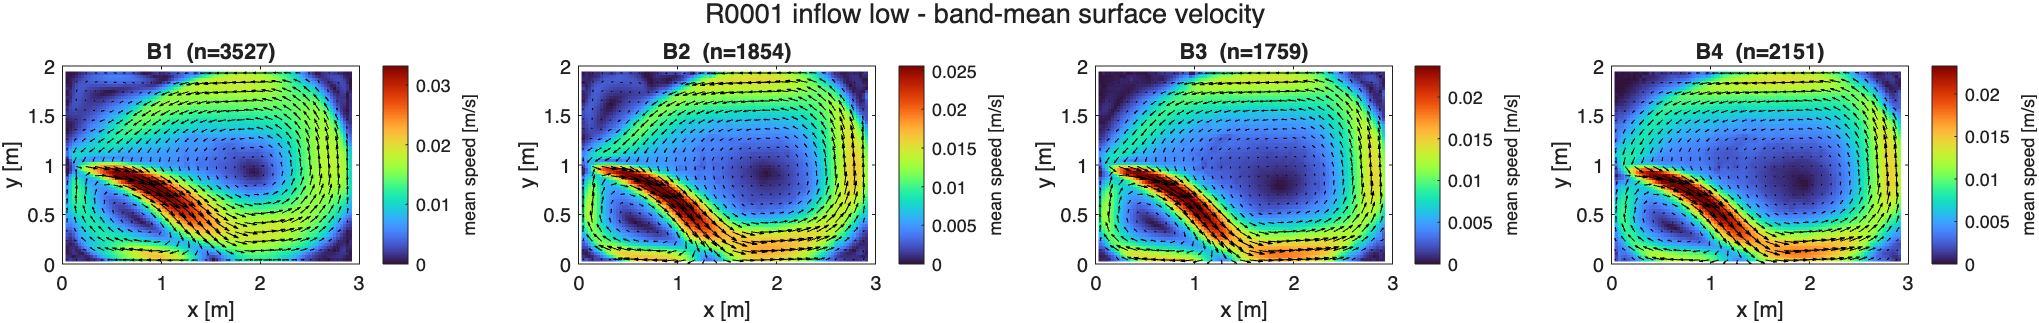
\includegraphics[width=\linewidth]{fig/R0001_band_mean_field.png}
\caption{Band-mean surface velocity fields for a representative inflow run
(R0001, low flow rate). One panel per depth band $B_1$--$B_4$ (shallow to
deep). Color: time-mean speed; vectors: mean velocity (auto-scaled per
panel). The port is at the center of the left short wall ($x=0$,
$y=\SI{1.0}{m}$).}
\label{fig:inflow_mean_field}
\end{figure}

inflow の代表的な帯平均表面速度場を Fig.~\ref{fig:inflow_mean_field} に示す. 全ての水深帯において, port から流入したジェットは port 軸($y = \SI{1.0}{m}$)に沿って直進せず, 片側(この run では $y$ 小側)の側壁へ明瞭に偏向し, 側壁に沿って加速したのち basin 全体を巡る大規模な非対称循環を形成した. 偏向側と反対側には低速の再循環域が広がる. この「偏向ジェット + 非対称循環」構造は 4 帯すべてで維持され, 水深帯によるトポロジーの切り替わりは認められなかった. この構造は, 浅い矩形貯水池で知られる非対称流レジーム \cite{dufresneClassificationFlowPatterns2010,camnasioExperimentalStudyVelocity2011}, および先行する可逆 port 実験の inflow 流況 \cite{mullerInfluenceOutflowSequences2012} と整合する.

スカラー指標の水深帯依存を条件横断で整理する(Fig.~\ref{fig:regime_comparison} も参照). まず運動強度 $E$ は, いずれの流量水準でも最浅帯 $B_1$ で最大となり, 潜没が進むにつれ単調に減少した(low: $2.5 \times 10^{-4} \to 9.3 \times 10^{-5}$~\si{m^2.s^{-2}}, high: $4.8 \times 10^{-3} \to 1.1 \times 10^{-3}$~\si{m^2.s^{-2}}). 同一流量で $B_1$ は $B_4$ の約 2.6--4.4 倍であり, 浅いほどジェットの運動量が表面近傍に集中することを反映する.

低流速域率 $\phi_{\mathrm{lv}}$($u_{\mathrm{th}} = 0.2\,U_p$)は逆に $h/a$ とともに単調増加した(low: $0.38 \to 0.58$, medium: $0.37 \to 0.58$, high: $0.22 \to 0.46$). すなわち, 潜没が進むほどジェットの表面影響域は狭まり, 静穏域が basin の過半を占めるようになる. 流量水準間では同一帯で high が最小の $\phi_{\mathrm{lv}}$ を示し, 相対閾値($u_{\mathrm{th}} \propto U_p$)にもかかわらず高流量ほどジェット影響域が相対的に広い.

左右非対称指標 $I_{\mathrm{asym}}$ は全帯・全流量で 0.22--0.30 の範囲にあり, $h/a$ にも流量にも系統的な依存を示さなかった. すなわち, 偏向ジェットに起因する左右不均衡は, 本実験の水深範囲では潜没度によらず頑健に存在する. 一方で run 間のばらつきは大きく, run 平均の $I_{\mathrm{asym}}$ は 0.16--0.37 に分布した. 同一条件の反復でも偏向の強さに幅があることは, 浅水池の非対称流に知られる双安定性・初期条件依存性 \cite{kantoushFLOWSHALLOWRECTANGULAR2008,dewalsExperimentalNumericalAnalysis2008} と整合的である. なお $I_{\mathrm{asym}}$ は定義上, 偏向の向きを畳んだ大きさである(Eq.~\eqref{eq:Iasym}). 偏向がどちら側に倒れるかは符号付き $I_{\mathrm{circ}}$ が担っており, Sec.~\ref{sec:results_branch} で扱う.

回転活動度 $I_{\mathrm{rot}}$ は $B_1$ で最大(0.095--0.123)となり, 潜没とともに約 0.06 へ減少した. $U_p$ で正規化しているため流量水準間でよく重なり($B_1$: low 0.102, medium 0.095, high 0.123), 正規化がスケーリングとして機能している. 一方, 符号付き循環指標 $I_{\mathrm{circ}}$ の絶対値は全 run・全帯で 0.013 以下, すなわち同一条件の $I_{\mathrm{rot}}$ の 1/10 以下にとどまった. 平均場(Fig.~\ref{fig:inflow_mean_field})が示すとおり inflow には強い回転運動が存在するから, この小ささは回転の不在ではなく, 偏向ジェットの主循環と反対側の再循環が符号付き面平均で大きく相殺した結果である. $I_{\mathrm{rot}} \gg |I_{\mathrm{circ}}|$ という組は「相殺する複数循環」の指標的シグネチャである.

ただし相殺は完全ではない. 残る正味の循環は run ごとに一方の符号へ明瞭に固定されており, その符号は本実験で最も系統的な流量依存を示す量であった. これは条件横断で平均すると消えてしまうため, 節を改めて run 単位で扱う(Sec.~\ref{sec:results_branch}).

非定常指標 $I_{\mathrm{unst}}(B_k)$ には, スカラー指標の中で最も明瞭な $h/a$ 遷移が現れた. $B_1$($h < a$)では 0.35--0.40 と大きな変動を示すのに対し, $B_2$($h/a \approx 1$)で 0.08--0.13 へ急減し, $B_3$, $B_4$($h/a > 1.09$)では 0.03--0.05 とほぼ定常となった. すなわち inflow の表面流は, port が自由表面と繋がる $h < a$ でのみ強い時間変動を伴い, 潜没の完了とともに急速に定常化する. この遷移は 3 流量水準すべてで同じ位置($B_1 \to B_2$)に現れ, $h/a \approx 1$ がレジームの転換帯であることを, 流況トポロジーではなく非定常性の観点から示す.

\subsection{Branch selection by flow rate}
\label{sec:results_branch}
% Results の中核: 流量が循環の符号を選ぶ. 符号つき I_circ は run 単位で扱う.

\begin{figure}[tb]
\centering
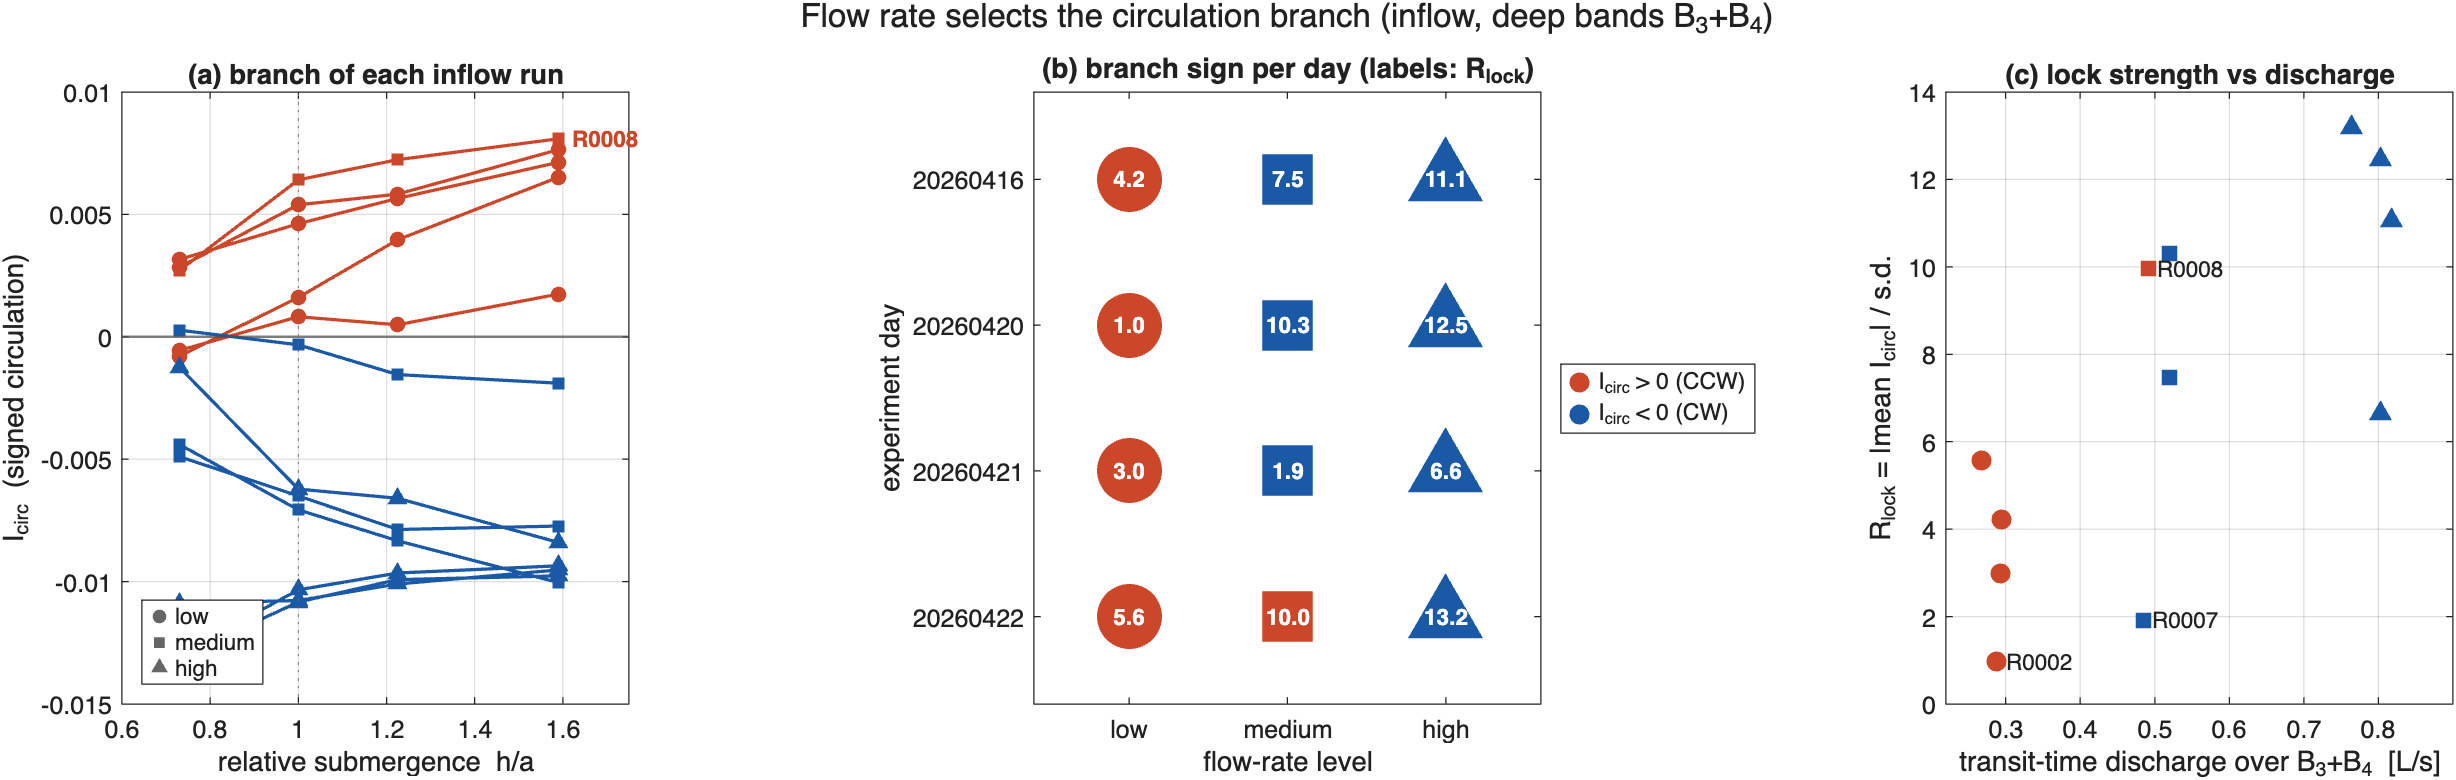
\includegraphics[width=\linewidth]{fig/fig_branch_selection.png}
\caption{Flow rate selects the circulation branch (inflow, 12 runs).
Colour: branch sign ($I_{\mathrm{circ}}>0$ counterclockwise, red;
$I_{\mathrm{circ}}<0$ clockwise, blue). Marker: flow-rate level (circle
low, square medium, triangle high). (a) Band-mean $I_{\mathrm{circ}}$
against relative submergence, one line per run; the dotted line marks
$h/a=1$. (b) Branch sign for each experiment day and flow level; labels
give $R_{\mathrm{lock}}$. Low is counterclockwise on all four days and
high is clockwise on all four days, so the sign splits within a single
day. (c) $R_{\mathrm{lock}}$ against the transit-time discharge over
$B_3+B_4$.}
\label{fig:branch_selection}
\end{figure}

前節でみたとおり inflow の平均場は片側へ偏向したジェットと非対称循環をもつ. その偏向がどちら側に倒れるかは, 対称な幾何配置の下では原理的に二つの等価な解(分枝)のいずれかであり, 個々の run の結果である. ここでは Sec.~\ref{sec:methods_metrics} の規約に従い, 深水帯 $B_3$, $B_4$ における符号付き $I_{\mathrm{circ}}$ を run ごとに評価した(Fig.~\ref{fig:branch_selection}).

第一に, 分枝の符号は流量水準によって系統的に分かれた. low の 4 run は 4/4 が正(反時計回り, ジェットは $y<y_{\mathrm{port}}$ 側の壁に付着), high の 4 run は 4/4 が負(時計回り)であり, 例外はない. medium のみが 3 負 / 1 正 に割れた. 帯別にみると(Fig.~\ref{fig:branch_selection}a), この符号は $h/a>1$ の帯で明瞭に確立する一方, 最浅帯 $B_1$ では 12 run 中 2 run(いずれも low)が深水帯と逆符号を示し, 正味循環そのものが小さい. すなわち分枝は, ジェットの潜没が完了するとともに定まる.

第二に, この符号の分かれ方は装置セットアップや日差では説明できない. inflow は 4 日間 $\times$ 3 水準の block 計画で実施しており(Sec.~\ref{sec:methods_facility}), Fig.~\ref{fig:branch_selection}b のとおり\textbf{同一日の中で} low と high の符号が必ず逆になる. 4 日間すべてでこの符号の対が再現するため, 分枝の選択は日ごとの初期条件や設営誤差ではなく, 流量に帰属する.

第三に, medium は二つの分枝が拮抗する遷移域であった. 逆符号を示した R0008 の流量は, 同水準の他 run と実質的に同じである. 水位ロガーの量子化に律速されない遷移時間法($Q=\Delta V_{B_k}/T_{B_k}$)で評価すると, 深水帯における実測流量は R0008 が \SI{0.492}{L/s}, 同符号側の R0007 が \SI{0.485}{L/s} で差は \SI{1.4}{\percent}(帯別では $B_3$ で \SI{3.2}{\percent}, $B_4$ で \SI{0.2}{\percent})にすぎず, medium 4 run 全体の散らばり(\SIrange{0.485}{0.519}{L/s})の中に収まる. したがって R0008 の逆符号は流量条件のずれでは説明できず, 同一条件下で二つの分枝がともに実現しうること(双安定性)を示す.

第四に, 分枝の固定の強さは流量とともに増大した(Fig.~\ref{fig:branch_selection}c). ロック強度 $R_{\mathrm{lock}}$ は low で 1.0--5.6, medium で 1.9--10.3, high で 6.6--13.2 であり, 水準の中央値は 3.6, 8.7, 11.8 と単調に増加する. 符号保持率でみても, 12 run 中 10 run では深水帯の全フレームが run 平均と同符号であり(保持率 1.000), 例外は最も弱い R0002(0.826)と, medium の遷移域にある R0007(0.970)のみであった. すなわち高流量ほど分枝は決定論的に選ばれ, かつ選ばれた後の保持も強い.

以上より, 本実験系では循環の\textbf{向き}が流量によって選択され, low と high では決定論的に, medium では双安定的に振る舞う. 流量は分枝の選択確率と固定の強さの双方を支配する制御パラメータとして機能している.

\subsection{Outflow flow regimes}
\label{sec:results_outflow}
% 非定常性を前景化しつつ, 分解能限界を明示する.

\begin{figure}[tb]
\centering
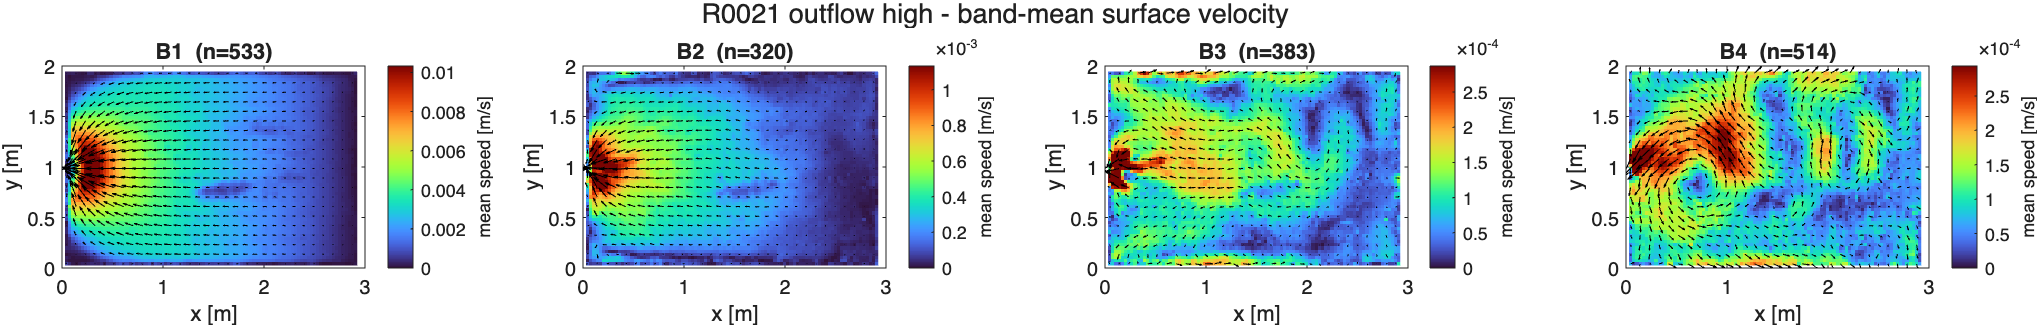
\includegraphics[width=\linewidth]{fig/R0021_band_mean_field.png}\\[2pt]
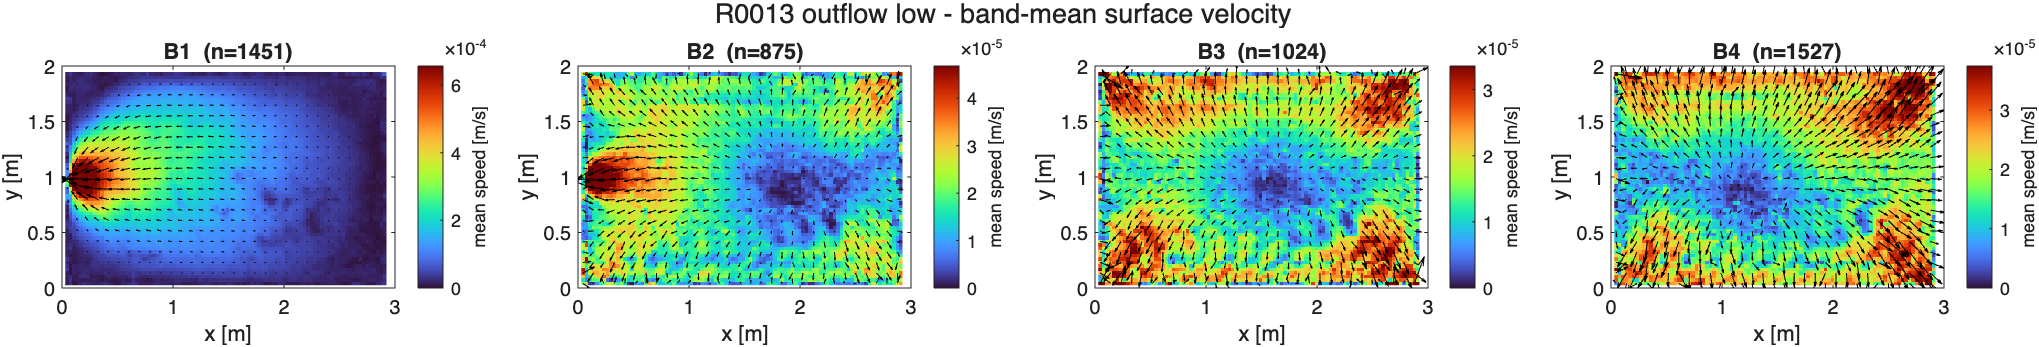
\includegraphics[width=\linewidth]{fig/R0013_band_mean_field.png}
\caption{Band-mean surface velocity fields for representative outflow runs.
Top: high flow rate (R0021). Bottom: low flow rate (R0013). Note the color
scales, two to three orders of magnitude smaller than in
Fig.~\ref{fig:inflow_mean_field}. Deep bands of the low-flow case
($B_2$--$B_4$, bottom) are below the PIV noise floor and show no coherent
mean structure.}
\label{fig:outflow_mean_field}
\end{figure}

outflow の代表的な帯平均表面速度場を Fig.~\ref{fig:outflow_mean_field} に示す. 十分に解像された条件(high の $B_1$ など)では, 表面流は basin 全域から port へ向かって収束する, 左右対称に近い「収束シンク」構造を示した. ベクトルは全域で port(左短辺中央)を向き, inflow に見られた偏向・再循環・卓越回転は認められない. 深い帯では平均構造そのものが微弱であり, low の $B_2$--$B_4$ では帯平均後もコヒーレントな構造を判読できなかった. これは前節の SNR 評価と整合し, outflow の深い条件では表面流速そのものが計測分解能以下であることを意味する.

ここで強調すべきは, 予備観察に基づき Introduction で言及した「outflow では basin 全体を占める単一循環」が, 静水から開始した本計測では確認されなかったことである. 静水開始の全 run において, outflow の表面流は(解像された範囲で)回転をもたない収束流であった. 指標でみても, outflow の $I_{\mathrm{rot}}$ は 0.002--0.007 と inflow(0.06--0.12)の約 1/20 にとどまり, $I_{\mathrm{circ}} \approx 0$ と併せて「相殺による正味 0」ではなく「回転の不在による 0」であることが裏づけられる. 予備観察で見られた単一循環は, 先行する inflow の残留循環に起因していた可能性が高い(Sec.~\ref{sec:discussion}).

低流速域率は全 outflow 条件で $\phi_{\mathrm{lv}} = 1.000$ に飽和した. すなわち表面の全域で流速が $0.2\,U_p$ を下回る. これは閾値の選択の問題ではなく(帯平均の表面流速は $U_p$ の 0.35--2.2\% であり, いかなる合理的な $\alpha$ でも飽和する), 「outflow では port の吸込みが自由表面の運動をほとんど駆動しない」という物理的所見である. 運動強度でみると, outflow の $E$ は同一流量の inflow より約 3 桁小さい.

非定常性は, 分解能の制約を踏まえ解像された帯に限って述べる. 唯一十分に解像された outflow high の $B_1$($\mathrm{SNR} \approx 37$)では $I_{\mathrm{unst}} = 0.76$ と, inflow の最大値($B_1$ の 0.35--0.40)の約 2 倍に達した. すなわち outflow の表面流は, 平均は微弱であるが, その弱い流れの相対変動は inflow より格段に大きい. この知見は, 取放水構造物近傍で「outflow の瞬時流速は時間平均の 3 倍超に達し, inflow は 0.9--1.1 倍にとどまる」と報告した Zhu らの観察 \cite{zhuExperimentalInvestigationUnsteady2023} と basin スケールで整合する. なお分解能限界の帯でも $I_{\mathrm{unst}}$ は 0.16--1.43 の大きな値を示すが, これらは noise floor 近傍の $E$ の比であり, ノイズ寄与と実変動を分離できないため定量的には解釈しない(Fig.~\ref{fig:regime_comparison} では白抜きマーカーで区別).

\subsection{Comparative regime transition and mode asymmetry}
\label{sec:results_comparison}
% Results の核: 同一軸比較と 4 つの要約.

\begin{figure}[tb]
\centering
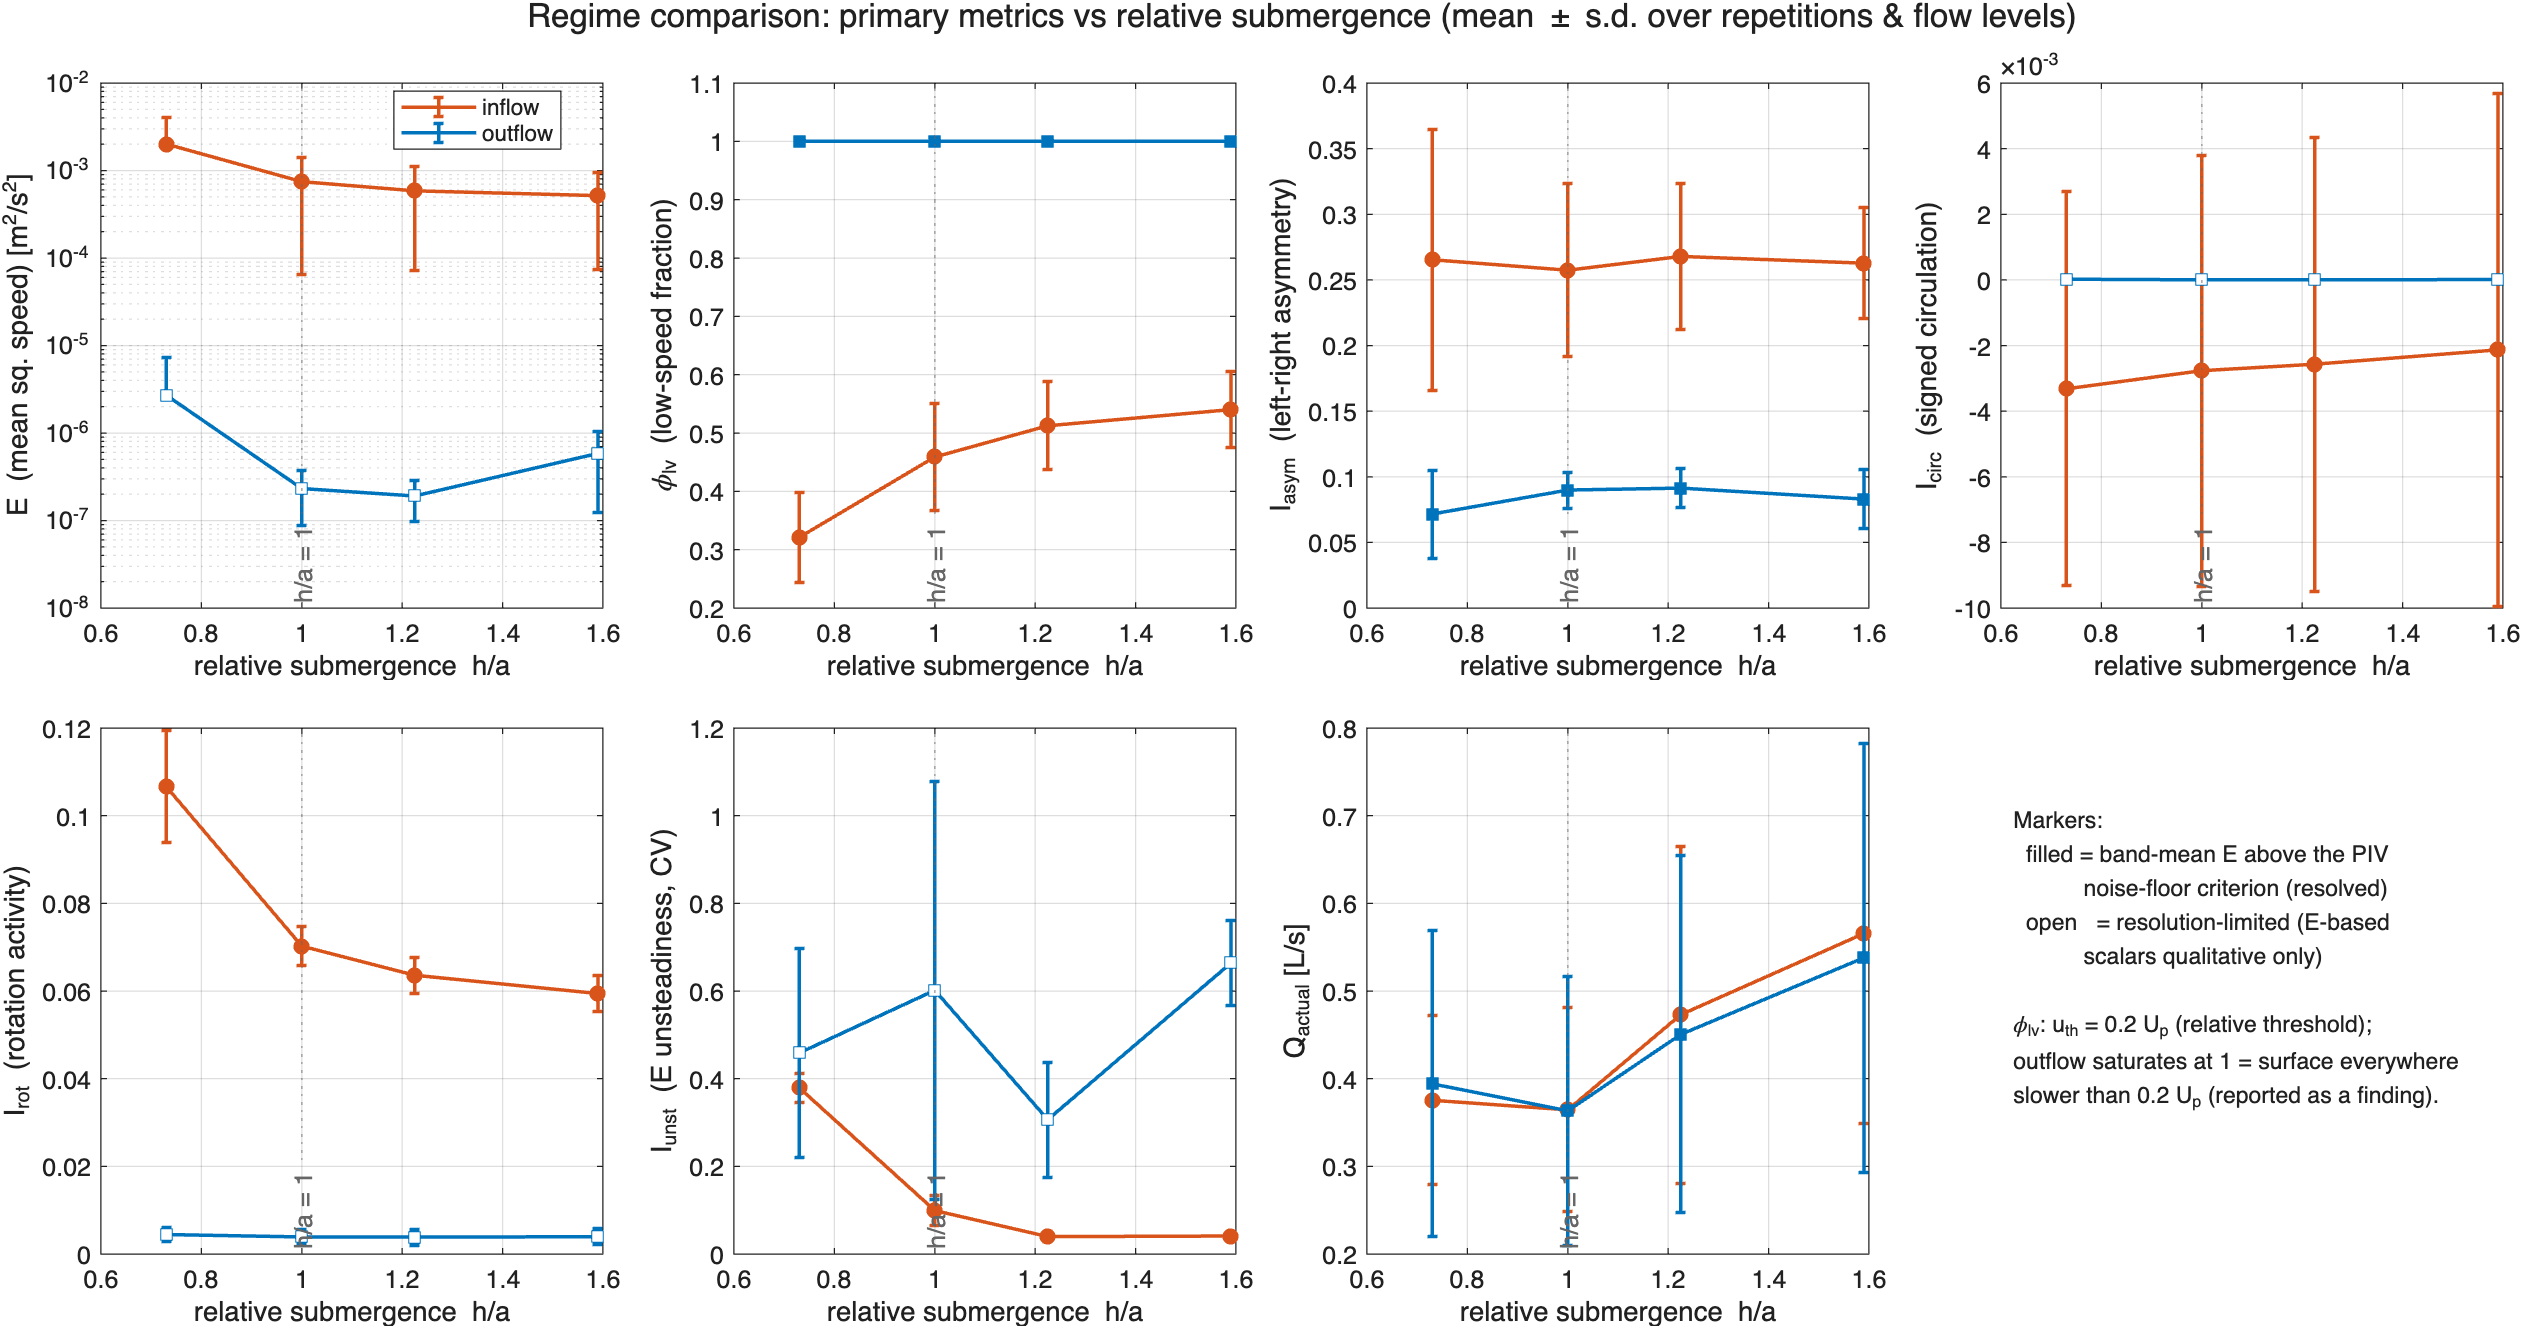
\includegraphics[width=\linewidth]{fig/fig_regime_comparison.png}
\caption{Primary metrics versus relative submergence $h/a$: inflow (orange
circles) versus outflow (blue squares). Symbols: mean over repetitions and
flow levels; bars: $\pm 1$ s.d. Open markers denote resolution-limited
bands ($\mathrm{SNR}<3$), whose $E$-based scalars are qualitative only.
The dotted line marks $h/a = 1$.}
\label{fig:regime_comparison}
\end{figure}

inflow と outflow を同一の $h/a$ 軸上で比較した結果を Fig.~\ref{fig:regime_comparison} に示す. 主要な知見は次の 4 点に要約される.

第一に, 同一の port 幾何を共有していても, inflow と outflow の表面流レジームは決定的に非対称である. トポロジーとしては「偏向ジェット + 非対称循環」(inflow)対「対称収束シンク」(outflow)であり, 指標としては $E$ で約 3 桁, $I_{\mathrm{asym}}$ で約 3 倍(0.26 対 0.08), $I_{\mathrm{rot}}$ で約 20 倍(0.06--0.12 対 0.002--0.007)の差に対応する. 非対称の向き(inflow が強く outflow が弱い)は, 深い貯水池模型 \cite{mullerInfluenceOutflowSequences2012} および実施設観測 \cite{mullerFlowFieldReservoir2018} と定性的に一致するが, その程度は本研究の浅い basin で著しく大きい(Sec.~\ref{sec:discussion}).

第二に, $h/a$ によるレジーム遷移は, 流況トポロジーの切り替えとしてではなく, 非定常性と表面影響度の変化として現れた. inflow のトポロジー(偏向ジェット + 循環)と outflow のトポロジー(収束シンク)はそれぞれ全水深帯で維持される一方, (i) inflow の $I_{\mathrm{unst}}$ は $h/a \approx 1$ を境に約 1 桁減少し, (ii) inflow の $\phi_{\mathrm{lv}}$ は $h/a$ とともに単調増加し(プール平均 $0.32 \to 0.54$), (iii) $E$ と $I_{\mathrm{rot}}$ も $B_1 \to B_2$ で最も大きく変化した. すなわち $h/a \approx 1$ は, 流れの「かたち」ではなく「強さ・不安定さ・表面への到達度」が切り替わる転換帯である.

第三に, 符号付き循環 $I_{\mathrm{circ}}$ はいずれの mode でも $I_{\mathrm{rot}}$ に比べて小さいが, その理由は正反対である. inflow は強い回転が大きく相殺した結果の小ささ($I_{\mathrm{rot}}$ 大)であり, outflow は回転が存在しないことによる小ささ($I_{\mathrm{rot}}$ 小)である. $(I_{\mathrm{circ}}, I_{\mathrm{rot}})$ の組でみることで初めて両者が区別される. さらに inflow では, 相殺しきらずに残る $I_{\mathrm{circ}}$ の符号が run ごとに固定され, その固定が流量に支配される(Sec.~\ref{sec:results_branch}). outflow にはこれに対応する分枝が存在しない.

第四に, 実流量 $Q$ は inflow と outflow でほぼ同一の水深依存(浅いほど小, 深いほど大)を示した. したがって上記のモード非対称は流量条件の差では説明できず, 同一流量における流入(運動量をもつジェットの注入)と流出(分布した吸込み)の力学的非対称そのものに帰着する.

以上を総合すると, 本実験で観察された表面流レジームは次のように整理される. inflow は全水深帯で「偏向ジェット + 非対称循環」レジームにあり, $h < a$ では加えて強い非定常性を伴う. またその循環の向きは, 潜没の完了とともに一方の分枝へ固定され, どちらの分枝が選ばれるかは流量に支配される. outflow は全水深帯で「対称収束シンク」レジームにあり, 表面運動は微弱だが相対変動は大きく, 分枝の選択という問題自体が生じない. Introduction で仮説とした 3 レジームのうち「basin 全体を占める単一循環」は静水開始条件では観察されず, 収束シンクが outflow の基本レジームである.
